\section{Entrega 2}



\subsection{Objetivo}

El objetivo de esta entrega es diseñar e integrar en el proyecto las mecánicas y métodos necesarios para crear las pruebas de las que constará el juego. Estos elementos son los que permitirán detectar y medir los movimientos del jugador para juzgar que la prueba se ha hecho de manera correcta.



\subsection{Iteración 1}

Se busca diseñar las técnicas básicas que se usarán para evaluar las pruebas. En concreto encontrar las herramientas que ofrecen Unity y VRTK y cual es la mejor forma de utilizarlas para detectar que los movimientos y las acciones del jugador son las adecuadas para cada una de las pruebas.

\subsubsection{Pruebas de posición}

Hay varias pruebas que dependen exclusivamente de la posición de los mandos en el espacio virtual, por lo que es esencial poder hacer un seguimiento de su posición en todo momento. Asignando una serie de posiciones para cada controlador durante la prueba y conociendo su posición real se podría determinar si el jugador está realizando el movimiento adecuado.

Unity trabaja con un sistema de coordenadas cartesianas y todos los objetos del juego tienen un atributo que indica su posición en dicho sistema (figura \ref{fig:E2_transform}), por lo que es sencillo obtener este dato.

\begin{figure}
  \centering
    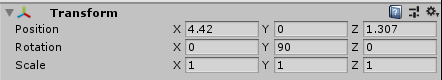
\includegraphics[width=0.9\textwidth]{04.Desarrollo/02.Entrega2/01.Iteracion2_1/00.Figuras/01.transform.png}
    \caption{Ejemplo del atributo Transform en Unity que representa la posición de un objeto en el espacio.}
    \label{fig:E2_transform}
\end{figure}

Por desgracia, no se puede basar el sistema únicamente en la posición exacta del mando, es necesario dar ciertos márgenes que ayuden al jugador a mantener el mando dentro de una zona que será tomada como válida. Una opción sería definir un punto del espacio y una distancia máxima a la que el mando se puede encontrar para considerarse una posición correcta. Unity incorpora de forma nativa un objeto llamado ‘trigger’. Un trigger (representado en la figura  \ref{fig:E2_transform}) se trata de un objeto en el espacio virtual, de cualquier forma o tamaño, que es completamente invisible al jugador y es capaz de detectar cuando otro objeto entra dentro de él. De esta forma, se puede definir un trigger en cualquier posición que reportará al sistema cuando el mando entra o sale de su perímetro.


\begin{figure}
  \centering
    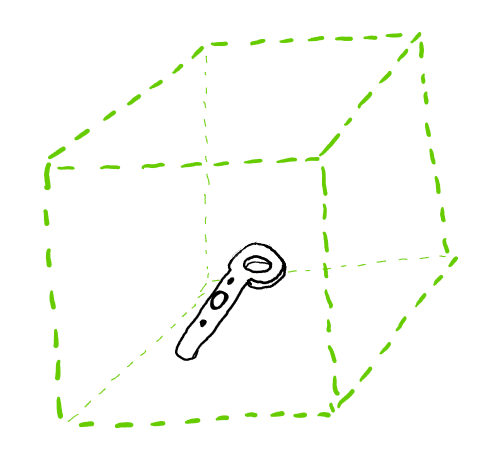
\includegraphics[width=0.5\textwidth]{04.Desarrollo/02.Entrega2/01.Iteracion2_1/00.Figuras/02.trigger.png}
    \caption{Boceto que muestra el uso de un trigger (cubo verde) para detectar el controlador en su interior.}
    \label{fig:E2_trigger}
\end{figure}


Teniendo la capacidad que ofrecen los trigger de Unity, definir las pruebas que se basan en la posición de las manos consiste en poder definir una serie de posiciones y tiempos en los que aparecerán dichos trigger para comprobar si el mando del jugador se encuentra en su interior. Puesto que los trigger son tratados como objetos comunes dentro de Unity, se pueden mover siguiendo una trayectoria y una velocidad, por lo que no solo pueden detectar posiciones, si no también evaluar el movimiento de los mandos entre dos puntos del espacio.

De esta forma ya se pueden definir algunas pruebas de movimiento:

\textbf{Posiciones.} En esta prueba se pide al jugador que adopte una pose concreta que aparece representada (figura \ref{fig:E2_poses}). Para este caso, para cada figura a imitar, es necesario definir una posición para cada mano, en dicha posición aparecerá un trigger. Si el jugador es capaz de colocar sus dos manos dentro de los trigger y mantenerlas en ellos, la prueba se dará como superada.


\begin{figure}
  \centering
    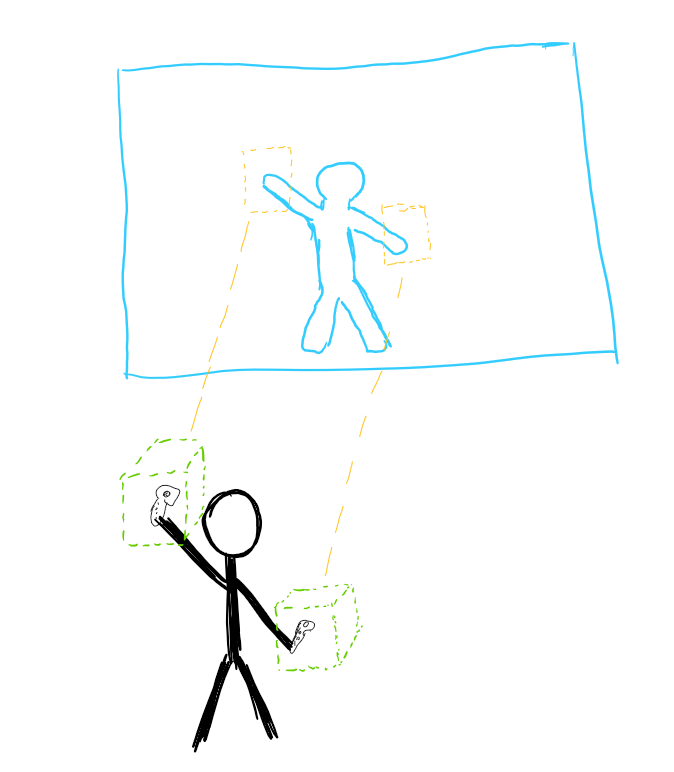
\includegraphics[width=0.5\textwidth]{04.Desarrollo/02.Entrega2/01.Iteracion2_1/00.Figuras/03.poses.png}
    \caption{Boceto que representa una posible prueba de figuras. En azul el modelo a seguir, en verde los trigger necesarios.}
    \label{fig:E2_poses}
\end{figure}

\textbf{Baile/movimientos.} (véase figura \ref{fig:E2_baile}) En este caso se puede definir un movimiento como la trayectoria que sigue un trigger dentro del espacio. Para ello es necesario definir un punto por cada momento intermedio, así como la velocidad a la que el trigger se moverá entre ellos. Si el jugador es capaz de mantener la mano dentro del espacio designado durante todo el movimiento la prueba habrá sido superada. En el caso de la prueba de baile, esta consiste en un conjunto de movimientos y posiciones uno tras otro.

\begin{figure}
  \centering
    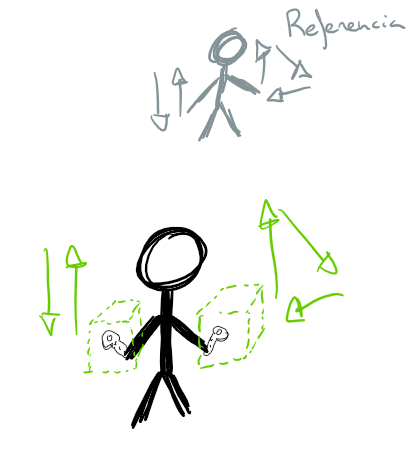
\includegraphics[width=0.5\textwidth]{04.Desarrollo/02.Entrega2/01.Iteracion2_1/00.Figuras/04.baile.png}
    \caption{Boceto representando una prueba de baile o movimientos. En gris la referencia a seguir, en verde los trigger y los movimientos que siguen.}
    \label{fig:E2_baile}
\end{figure}


\textbf{Objetivos.} Esta prueba hace que el jugador vea como varios objetos se aproximan hacia él y debe tocarlos con la mano conforme llegan a su posición, según se observa en la figura \ref{fig:E2_objetivos}. Cada objeto puede tener dos colores, el cual indica al jugador con qué mano debe tocarlo. Los objetos de color rojo se acercarán al jugador por su lado izquierdo y deberá tocarlos con su mano izquierda. Los objetos azules actuarán de la misma forma, pero para el lado derecho. Cada uno de estos objetos tendrá un ‘collider’ que es equivalente a un trigger, pero para objetos visibles al jugador, esto permitirá determinar si el jugador ha realizado la prueba de forma correcta.


\begin{figure}
  \centering
    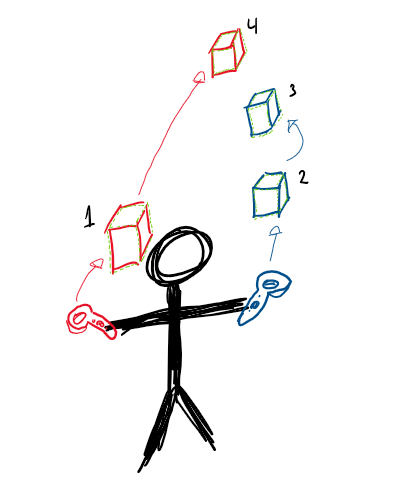
\includegraphics[width=0.5\textwidth]{04.Desarrollo/02.Entrega2/01.Iteracion2_1/00.Figuras/05.objetivos.png}
    \caption{Boceto de una prueba de objetivos. Los objetivos en azul y rojo deberán tocarse con el mando del mismo color.}
    \label{fig:E2_objetivos}
\end{figure}


\subsubsection{Pruebas de interacción}

Algunas de las pruebas requerirán que el jugador interactúe con objetos virtuales, cogiéndolos, soltándolos o de formas similares. Por suerte, estas son capacidades básicas que ofrecen SteamVR y VRTK y que ya fueron integradas en el proyecto como parte de la primera entrega. Por lo que la definición de cada prueba consistirá en gran parte de la generación de los objetos virtuales: cuáles, dónde y cómo aparecen. Así como detectar lo que el jugador hace con ellos.

Para la prueba de agrupación de objetos (véase figura \ref{fig:E2_agrupacion}) se presentarán al jugador un grupo de objetos virtuales y esté deberá descubrir su asociación y colocarlos en dos zonas separadas. Estas zonas se pueden definir usando los trigger explicados anteriormente, de modo que basta con detectar cuándo todos los objetos han sido introducidos en alguna de las dos zonas, y evaluar si cada uno está donde le corresponde.


\begin{figure}
  \centering
    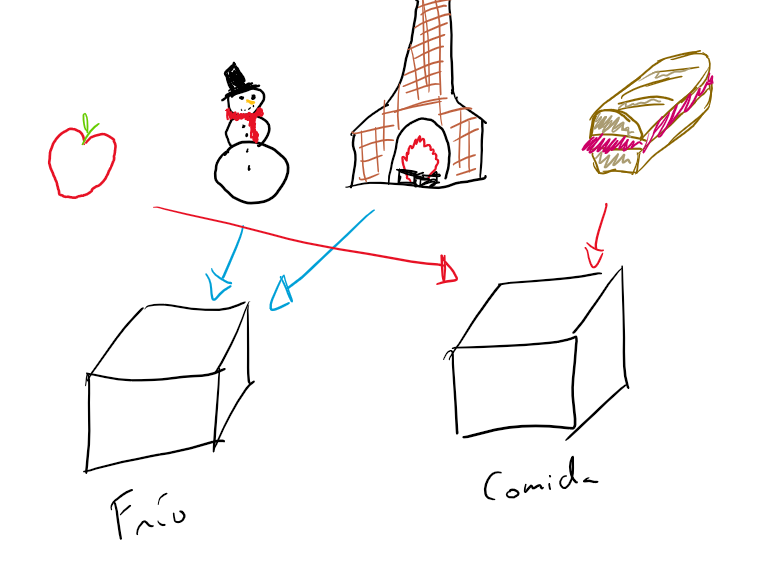
\includegraphics[width=0.5\textwidth]{04.Desarrollo/02.Entrega2/01.Iteracion2_1/00.Figuras/06.agrupacion.png}
    \caption{Boceto de la prueba de agrupación de objetos. Las categorías "frío" y "comida" no son visibles para el jugador.}
    \label{fig:E2_agrupacion}
\end{figure}

En la prueba de figuras superpuestas se mostrarán al jugador un conjunto de objetos virtuales o siluetas que se encuentran superpuestos unos con otros como se muestra en la figura \ref{fig:E2_superpuestas}. El jugador deberá averiguar de qué objetos de trata y responder seleccionando la respuesta correcta entre las disponibles que se presentarán mediante botones interactivos en RV. La funcionalidad de estos botones está proporcionada por los paquetes instalados en la entrega anterior.


\begin{figure}
  \centering
    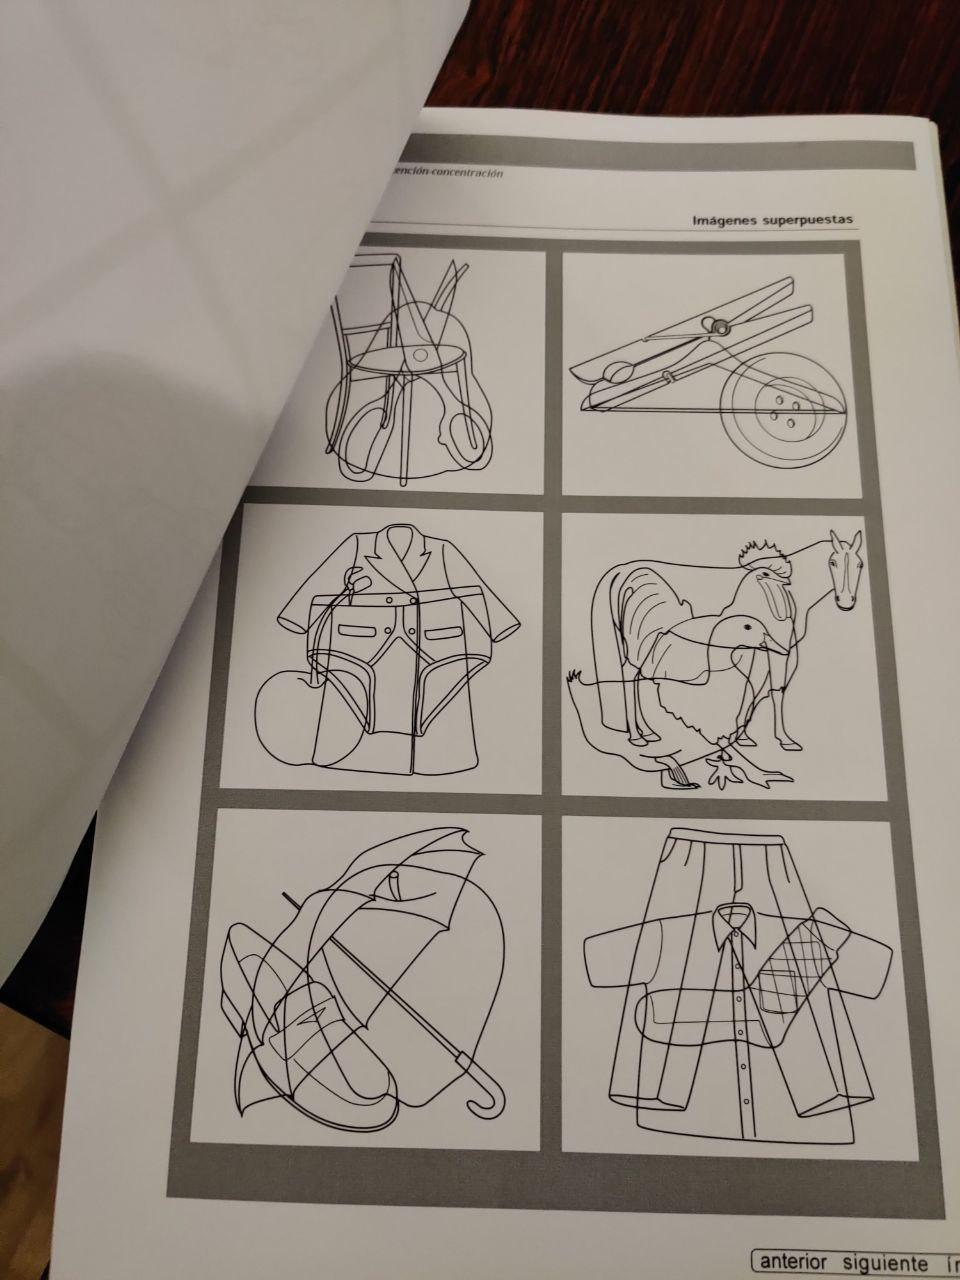
\includegraphics[width=0.5\textwidth]{04.Desarrollo/02.Entrega2/01.Iteracion2_1/00.Figuras/07.superpuestas.jpg}
    \caption{Fotografía de un ejercicio de figuras superpuestas en formato de papel.}
    \label{fig:E2_superpuestas}
\end{figure}

Para la prueba de asociación de sonidos se presentan una serie de objetos al jugador de la misma forma que en la prueba de agrupación de objetos, pero en este caso el jugador deberá escuchar un sonido y decidir qué objeto es el que produce dicho sonido, como se ilustra en la figura \ref{fig:E2_sonidos}. La única diferencia entre esta prueba y la de agrupación es que es necesario crear un objeto que sea capaz de reproducir un sonido previamente grabado y hacer que el jugador lo oiga. Por suerte esta es una funcionalidad básica de Unity.


\begin{figure}
  \centering
    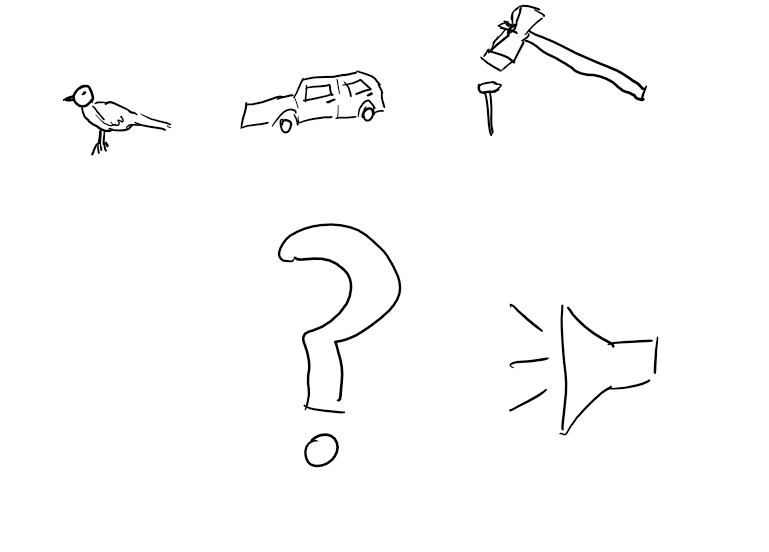
\includegraphics[width=0.5\textwidth]{04.Desarrollo/02.Entrega2/01.Iteracion2_1/00.Figuras/08.sonidos.png}
    \caption{Boceto que representa la prueba de asociación de un sonido con el objeto que lo produce.}
    \label{fig:E2_sonidos}
\end{figure}


Finalmente, para la prueba de localización de sonidos únicamente es necesario colocar un emisor de sonido en un punto del espacio rodeando al jugador. Unity es capaz de utilizar audio ambisónico, un tipo de sonido que permite al usuario localizar el punto exacto en el espacio de donde proviene dicho sonido. Por tanto, se usará esta tecnología para hacer que el jugador se gire en la dirección correcta de la que proviene el sonido. Cuando el jugador sea capaz de ver el objeto que producía el sonido, la prueba ha sido superada. 


\subsubsection{Pruebas de entorno}


Estas son las pruebas en las que no se requiere que el jugador interactúe con el entorno de manera directa. Se presenta un entorno que el jugador debe observar y escuchar. Por tanto, para la evaluación de este tipo de pruebas es necesaria la participación de una persona externa al juego, preferiblemente una persona experta en entrenamiento cognitivo que actúe de guía para el usuario. Para estas pruebas no es necesario el uso de ninguna mecánica especial salvo la generación de los objetos virtuales del entorno.





\subsection{Iteración 2}

En esta iteración se busca crear en Unity las mecánicas básicas necesarias para realizar las distintas pruebas.


\subsubsection{Pruebas de posición} 
\label{E2_triggers}

Para implementar los triggers explicados en la iteración anterior se ha creado un objeto en Unity con forma de cubo y un tamaño que equivaldría a 50x50x50 centímetros en el mundo real. Durante el desarrollo del proyecto los triggers serán visibles para facilitar el trabajo, y serán de color rojo por defecto, pero se volverán verdes cuando detecten un mando en su interior, mostrando así su correcto funcionamiento.

Cada trigger contiene un único script que define su comportamiento durante el juego y es el encargado de detectar si hay un mando en su interior y reflejarlo de forma adecuada. El script utiliza las cinco variables mostradas en la figura \ref{fig:E2_variablesTriggers}, dos de ellas (‘correctMaterial’ e ‘incorrectMaterial’) son para almacenar los materiales que mostrará según haya o no algún mando en su interior. ‘controllerTag’ contiene el texto con el que se van a etiquetar los mandos, para de esta forma poder detectar si el objeto dentro del trigger es un mando. ‘nControllers’ almacena en todo momento el número de mandos que hay dentro del trigger, ya que es posible que haya varios en un mismo instante. Finalmente, ‘controllerInside’ contendrá un valor de verdadero o falso según haya algún mando en el trigger o no.


\begin{figure}
  \centering
    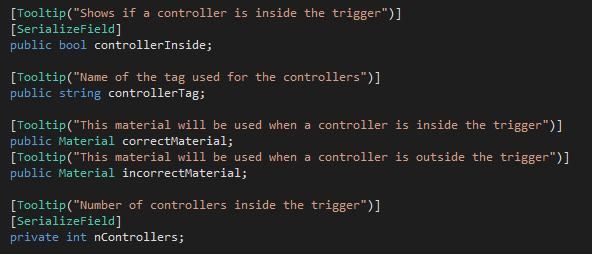
\includegraphics[width=0.9\textwidth]{04.Desarrollo/02.Entrega2/02.Iteracion2_2/00.Figuras/01.variables_trigger.png}
    \caption{Variables en el script para los triggers.}
    \label{fig:E2_variablesTriggers}
\end{figure}

Durante el juego este script detecta la entrada y salida de cualquier objeto en el trigger mediante dos funciones nativas de Unity: OnTriggerEnter y OnTriggerExit, como se muestra en la figura \ref{fig:E2_onTriggerEnter}. Las funciones se activan cuando se detecta un cualquier nuevo objeto, por lo que es necesario distinguir si se trata de un mando o no, para ello se utiliza la etiqueta “Controller” que está almacenada en la variable controllerTag. Si la etiqueta es la adecuada, quiere decir que un mando ha entrado o salido del trigger, por tanto, se actualiza el número de mandos que hay actualmente dentro del mismo.


\begin{figure}
  \centering
    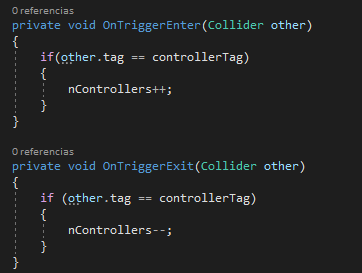
\includegraphics[width=0.7\textwidth]{04.Desarrollo/02.Entrega2/02.Iteracion2_2/00.Figuras/02.on_trigger_enter.png}
    \caption{Métodos para manejar la entrada y salida de objetos en un trigger.}
    \label{fig:E2_onTriggerEnter}
\end{figure}

Finalmente, el script comprobará de forma constante el número de mandos en su interior (figura \ref{fig:E2_updateTrigger}), en caso de no haber ninguno, pondrá la variable ‘controllerInside’ a falso y usará el material rojo, indicando que no hay mandos en su interior. En caso contrario, el trigger usará el material ‘correctMaterial’ para mostrar que hay al menos un mando en él, así como activar la variable ‘controllerInside’. Por último, como medida de seguridad se comprueba que el número de mandos dentro del trigger no sea menor que 0 ni mayor que 2, y en caso de darse dicha situación, reasigna el valor a 0 si era menor que 0 o a 2 si era mayor que 2.


\begin{figure}
  \centering
    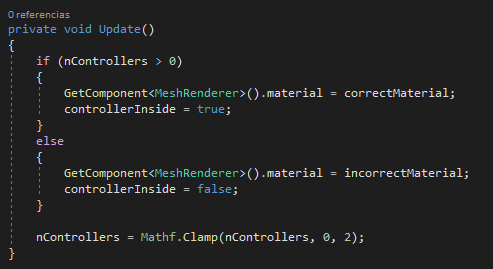
\includegraphics[width=0.7\textwidth]{04.Desarrollo/02.Entrega2/02.Iteracion2_2/00.Figuras/03.update_trigger.png}
    \caption{Parte del script que controla el número de mandos dentro de un trigger.}
    \label{fig:E2_updateTrigger}
\end{figure}

El siguiente problema planteado es la posición de los triggers en el espacio de juego.  Los triggers deben estar en una posición fija con relación al jugador, pero debido a la naturaleza de la realidad virtual, el jugador puede moverse y rotar libremente, lo que podría causar que los triggers no se encuentren en el lugar esperado por el jugador. Para solucionar este problema se ha diseñado una matriz de posiciones posibles en las que puede aparecer un trigger (mostrada en la figura \ref{fig:E2_spawnArray}), y esta matriz se encuentra ligada a la posición del jugador y se mueve junto a él. De este modo los triggers siempre aparecen en el mismo lugar con respecto al jugador.


\begin{figure}
  \centering
    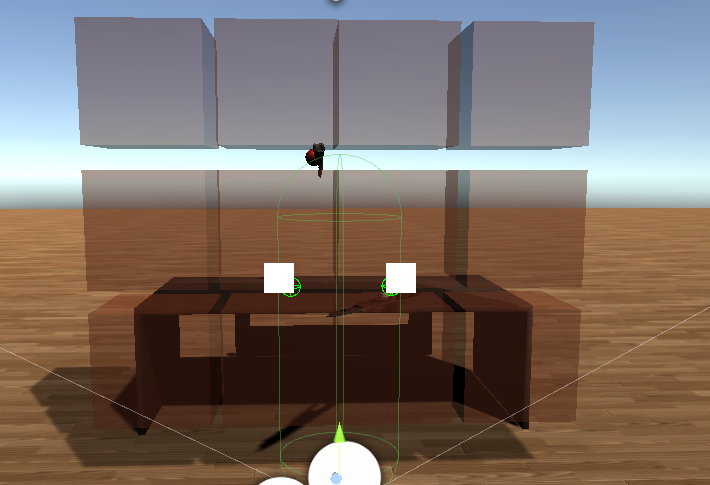
\includegraphics[width=0.7\textwidth]{04.Desarrollo/02.Entrega2/02.Iteracion2_2/00.Figuras/04.spawn_array.png}
    \caption{Representación de la matriz con 3 filas y 4 columnas de triggers. En el centro, una capsula verde representa al jugador, y los cubos blancos sus manos.}
    \label{fig:E2_spawnArray}
\end{figure}

A continuación, es necesaria una forma de crear los triggers necesarios para cada nivel en su posición correcta, así como un método para expresar la posición de cada trigger para cada nivel. Como primera solución a este problema se ha optado por diseñar usando JSON una forma de expresar las posiciones de la matriz que deben estar ocupadas por un trigger, usando un objeto en Unity capaz de leer dicho formato desde un fichero y cargar los triggers necesarios en el entorno virtual.

El formato elegido para la representación de un nivel en JSON se muestra en la figura \ref{fig:E2_json} y está compuesto por un campo “level” que encapsula todos los datos y contiene una lista de secciones llamada “part”. Cada sección corresponde a un estado concreto de la matriz de triggers, y cada uno de esos estados está definido por un “time” que indica cuantos segundos tardará en activarse dicho estado desde el comienzo de la prueba; y una matriz “triggerPositions” que contiene valores true/false dónde un ‘true’ significa que el trigger que ocupa dicha posición de la matriz estará activo y un false significa que no habrá ningún trigger en dicha posición.


\begin{figure}
  \centering
    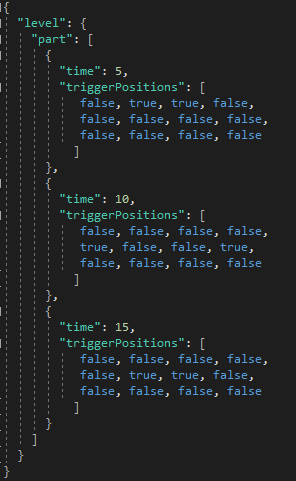
\includegraphics[width=0.4\textwidth]{04.Desarrollo/02.Entrega2/02.Iteracion2_2/00.Figuras/05.json.png}
    \caption{Ejemplo de la estructura JSON representando un nivel con 3 partes.}
    \label{fig:E2_json}
\end{figure}


En el ejemplo presentado en la figura 13 se muestra un nivel que empieza sin ningún trigger activo, a los 5 segundos del comienzo de la prueba se crean los dos triggers centrales de la primera fila. Pasados 10 segundos desde el comienzo, se desactivan los triggers anteriores y se activan los dos más exteriores de la fila central. Cinco segundos después se cargan los triggers finales, los centrales de la segunda fila.

Para las pruebas que requieren el movimiento de los mandos de un punto a otro, se puede crear un trigger aislado que siga una trayectoria a una velocidad determinada, pero teniendo este sistema de gestión de los triggers mediante una matriz y la capacidad de cargar mediante un fichero diferentes configuraciones de la misma que se modifiquen en momentos determinados, se puede modificar el procedimiento para las pruebas de movimiento de forma que se adapten a este sistema y faciliten el desarrollo del proyecto.

Con el primer diseño es necesario definir un punto de inicio del trigger (con los problemas respecto a su posición relativa explicados anteriormente), así como una serie de puntos intermedios junto con un tiempo que debe tardar el trigger en alcanzarlos. Usando el diseño desarrollado para los triggers estáticos se logra resolver tanto los problemas de posición relativa, mediante el uso de la matriz que sigue al jugador, como el problema del tiempo entre cada punto intermedio gracias a que se puede definir en el fichero el momento en el que aparecerá cada trigger. El único impedimento restante es contabilizar de manera correcta el movimiento del usuario de un trigger al siguiente con una velocidad adecuada. Para ello, el objeto controlador de la prueba se encarga de contar el tiempo que el jugador está fuera del trigger entre la primer y la segunda posición, de esta forma, se puede averiguar si el movimiento del jugador ha sido fluido y acorde a lo esperado. 

Esta solución para las pruebas de movimiento es menos precisa que la original, pero permite una mayor simplicidad y modularidad a la hora de construir niveles ya que se basa en el sistema desarrollado anteriormente.


\subsubsection{Pruebas de interacción}


Para este tipo de pruebas se diseñó en primer lugar utilizar los mismos triggers que se han usado hasta el momento, pero durante la implementación se ha encontrado una funcionalidad de VRTK que se ajusta más al resultado deseado: ‘InteractableSnapZone’. Estos son objetos que forman una zona en la que si se coloca un objeto, cuando se suelte dicho objeto este se moverá automáticamente para colocarse en una posición y orientación determinada (figura \ref{fig:E2_snapHighLights}) de forma que el objeto queda siempre colocado de la misma forma. Además, ofrece esta funcionalidad con un rango de acción variable, es decir, la distancia desde la cual será capaz de colocar un objeto en el lugar adecuado. 


\begin{figure}
  \centering
    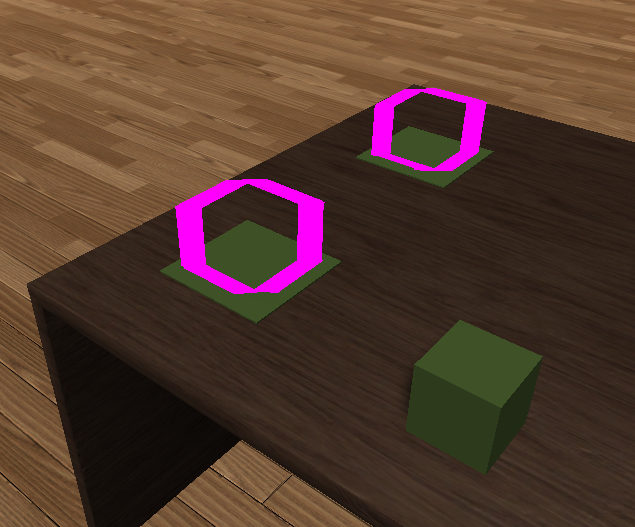
\includegraphics[width=0.5\textwidth]{04.Desarrollo/02.Entrega2/02.Iteracion2_2/00.Figuras/06.snap_highlights.png}
    \caption{Ejemplo que muestra dos plataformas verdes con dos InteractableSnapZone. En rosa se remarca la posición que ocupará el cubo verde si se suelta dentro de una de dichas zonas.}
    \label{fig:E2_snapHighLights}
\end{figure}

En la prueba de agrupación de objectos, que consiste en que al jugador se le presentan una serie de objetos y tiene que clasificarlos en dos grupos moviéndolos y colocándolos en sus zonas correspondientes, se usan dos zonas de snap y mediante un script se puede comprobar qué objetos hay en cada zona.


\begin{figure}
  \centering
    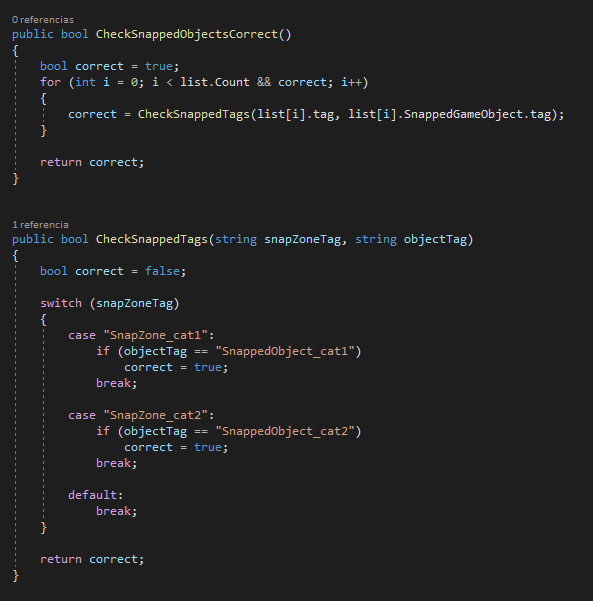
\includegraphics[width=0.8\textwidth]{04.Desarrollo/02.Entrega2/02.Iteracion2_2/00.Figuras/07.script_snap.png}
    \caption{Dos métodos del script que controla los objectos dentro de cada snap zone.}
    \label{fig:E2_scriptSnap}
\end{figure}

En el script presentado en la figura \ref{fig:E2_scriptSnap} aparecen dos de las funciones utilizadas para comprobar que cada snap zone contiene un objeto de la categoría que se desea. El método CheckSnappedObjectsCorrect recorre la lista ‘list’ que contiene todos los snap zones del nivel y para cada zona que hay en el nivel comprueba que tiene dentro un objeto de una categoría válida mediante la función CheckSnappedTags. Esta función compara la etiqueta que describe a la zona de snap con la etiqueta que describe al objeto de su interior, y en caso de ser de la misma categoría (en el ejemplo: cat1 o cat2), devuelve un valor verdadero que indica al controlador que el objeto es válido. Si existe alguna zona que contenga un objeto no válido, se da la prueba por fallida, pero en caso contrario la prueba habrá sido superada.

Para las pruebas de objetos superpuestos y de asociación de sonidos se utiliza un botón que el jugador tendrá que pulsar para indicar la respuesta correcta. La funcionalidad básica de los botones viene dada por SteamVR y consiste en un objeto que el jugador puede mover en un eje empujándolo con la mano (figura \ref{fig:E2_boton}). En este caso no es necesario agarrar el botón o interactuar de forma explícita con él, basta con que el jugador lo empuje para que el botón se active y ejecute un script, que es este caso indica si el botón pulsado es el correcto.


\begin{figure}
  \centering
    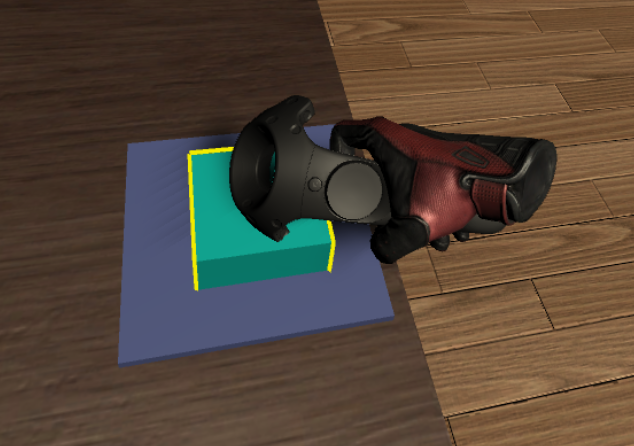
\includegraphics[width=0.5\textwidth]{04.Desarrollo/02.Entrega2/02.Iteracion2_2/00.Figuras/08.boton.png}
    \caption{Jugador pulsando un botón.}
    \label{fig:E2_boton}
\end{figure}

Finalmente, para la prueba de localización de sonidos se utiliza la capacidad que tiene Unity para generar audio 3D mediante el uso de su fuente de audio (figura \ref{fig:E2_audioSource}) junto con el espacializador de Oculus que es necesario configurar como se muestra en la figura \ref{fig:E2_audioSpatializer}. De esta forma solo en necesario colocar una fuente de sonido en cualquier punto alrededor del jugador y comprobar si está mirando hacia el origen del audio. Para hacer esta comprobación se usa una función del motor de renderizado de Unity que permite saber si un objeto va a ser dibujado en pantalla o no. Puesto que los objetos no visibles no se dibujan, de esta manera se determina si el jugador está viendo la fuente de audio mediante un sencillo script mostrado en la figura \ref{fig:E2_audioVisible}.

\begin{figure}
  \centering
    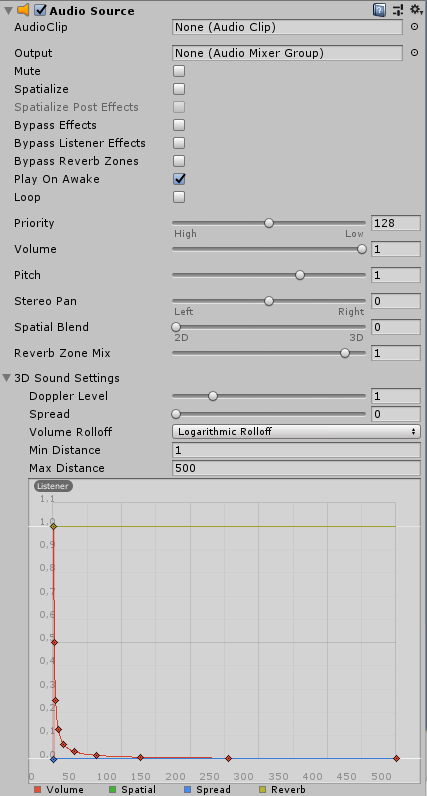
\includegraphics[width=0.5\textwidth]{04.Desarrollo/02.Entrega2/02.Iteracion2_2/00.Figuras/09.audio_source.png}
    \caption{Muestra de la configuración de una fuente de audio en Unity.}
    \label{fig:E2_audioSource}
\end{figure}

\begin{figure}
  \centering
    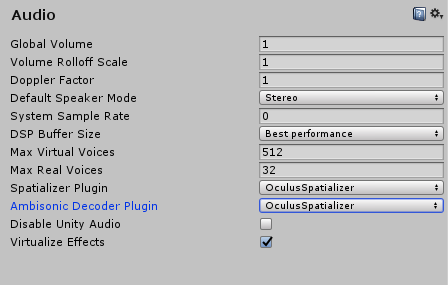
\includegraphics[width=0.5\textwidth]{04.Desarrollo/02.Entrega2/02.Iteracion2_2/00.Figuras/10.audio_spatializer.png}
    \caption{Ventana de configuración en la que es necesaria seleccionar OculusSpatializer para utilizar el sonido 3D.}
    \label{fig:E2_audioSpatializer}
\end{figure}

\begin{figure}
  \centering
    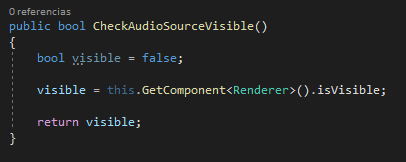
\includegraphics[width=0.5\textwidth]{04.Desarrollo/02.Entrega2/02.Iteracion2_2/00.Figuras/11.audio_visible_script.png}
    \caption{Método que comprueba si la fuente de audio es visible por el jugador. Este script debe estar en la propia fuente.}
    \label{fig:E2_audioVisible}
\end{figure}

Con esto quedan implementadas en el proyecto todas las mecánicas básicas que son necesarias para comprobar si el jugador realiza las pruebas de manera correcta o no.




\subsection{Iteración 3}

En la última iteración de esta entrega se ha buscado poner a prueba la adaptación de varias personas al uso de la realidad virtual en general y en concreto a las mecánicas desarrolladas en esta entrega. Se ha hecho hincapié en la facilidad de uso y la comodidad del usuario durante el juego. 

Para esto se ha desarrollado una pequeña escena de prueba en la que primero el jugador debe adoptar una postura corporal de forma que se activen de forma correcta unos triggers preparados previamente y que cambian cada 10 segundos hasta 3 veces. A continuación, el usuario se encuentra ante una mesa virtual (figura \ref{fig:E2_mesa}) en la que encuentra varios objetos, dos cubos verdes y dos cubos azules. En los bordes de la mesa hay 4 plataformas de los mismos colores que los cubos. El jugador puede interactuar libremente con estos objetos, pero debe colocar cada cubo en una plataforma de su color correspondiente. Una vez realizada la tarea, debe pulsar el botón situada en la parte derecha de la mesa. La pulsación de este botón provoca que se reproduzca un sonido proveniente de la parte trasera del usuario. Finalmente, el jugador tiene que girarse para ver la fuente del sonido y terminar así la prueba.


\begin{figure}
  \centering
    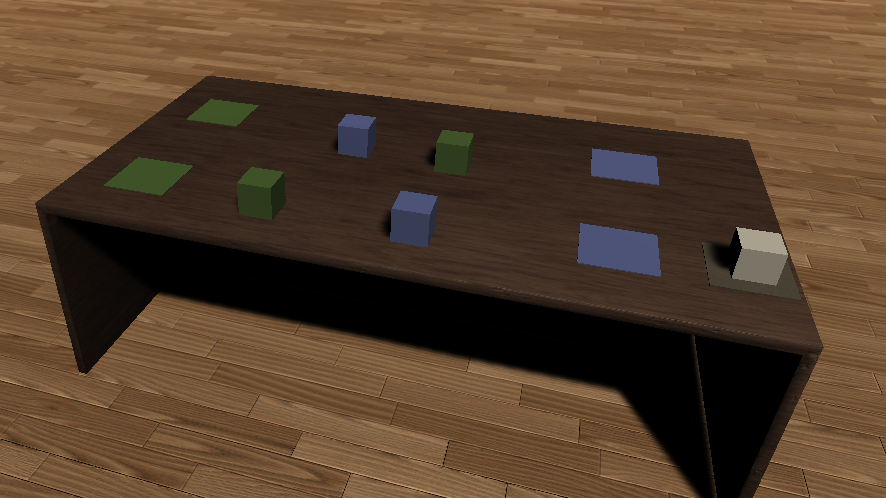
\includegraphics[width=0.5\textwidth]{04.Desarrollo/02.Entrega2/03.Iteracion2_3/00.Figuras/01.mesa.png}
    \caption{Mesa con objetos de prueba para las interacciones básicas, snap zones y botones.}
    \label{fig:E2_mesa}
\end{figure}




Esta prueba se ha realizado con varias personas mientras se monitorizaba mediante Unity todos los resultados y el funcionamiento de las mecánicas. Han participado tres personas que se caracterizan de la siguiente forma:

\begin{itemize}
    \item{Persona mayor de 50 años con poca experiencia tecnológica y ninguna experiencia en RV.}
    \item{Persona entre 20 y 25 años, con experiencia tecnológica, pero sin experiencia en RV.}
    \item{Persona entre 20 y 25 años con gran experiencia tanto en tecnología como en RV.}
\end{itemize}




Tras guiar a estas tres personas durante la prueba y posteriormente entrevistarlas sobre su experiencia se han obtenido información útil para el desarrollo del proyecto y que se expone a continuación.

\begin{itemize}

\item{Todas las personas han necesitado un breve periodo de adaptación a la realidad virtual, en el caso de las personas jóvenes ha sido más corto y ha consistido principalmente en ajustes físicos del casco de realidad virtual como la tensión se sus amarres o la distancia focal de las lentes para evitar ver de forma borrosa. En la persona mayor ha sido necesario más tiempo para adaptarse al entorno virtual, pero no provocando mareo ni otros efectos perjudiciales.}
\item{Aunque ninguna persona ha tenido dificultades en seguir la prueba de posiciones, se ha observado que es necesario reajustar el tamaño y posición de los triggers, así como su cantidad y separación.}
\item{En el uso de las manos virtuales las dos personas sin experiencia en RV prefieren que el avatar muestre una representación virtual del mando que están sosteniendo para facilitar la inmersión. Sin embargo, a la hora de interactuar y coger objetos han encontrado más difícil utilizar el avatar con mando por la discordancia con el mundo real en el que no se puede coger otro objeto mientras ya se tiene uno sujeto. La persona con experiencia en RV ha preferido el avatar sin representación del mando en todo momento. Por tanto, se concluye que el mando virtual es útil para crear una inmersión inicial, pero debe ser sustituido cuando llega el momento de realizar interacciones con las manos.}
\item{Durante la prueba de agrupación de los objetos por colores, las dos personas sin experiencia en RV han tenido ligeros inconvenientes a la hora de coger objetos principalmente por la estimación de la distancia a la que se encuentran. Estos inconvenientes no han sido graves y ambas personas se han acostumbrado rápidamente.}
\item{Llegado el momento de intentar localizar la posición de la fuente de sonido a sus espaldas todo el mundo ha tenido problemas en discernir de dónde procedía el sonido. Tras investigar el problema es posible que por la naturaleza del audio digital y el dispositivo de reproducción usado sea difícil distinguir entre ciertas posiciones de una fuente como por ejemplo detrás del jugador o justo sobre su cabeza. Por lo tanto, esta prueba deberá ser acotada para que la fuente de sonido solo pueda apareces en lugares en los que sea posible localizarla de forma cómoda.}

\end{itemize}







\subsection{Conclusiones de la entrega}


Para la creación y diseño de las pruebas se han tenido en cuenta tres bases: ejercicios ya existentes y que se utilizan en entrenamiento cognitivo en la actualidad, interacciones sacadas de la ambientación deseada del juego (concurso de TV) y conceptos de juegos y experiencias de RV actuales que no tienen relación con el entrenamiento cognitivo.
De esta forma se ha buscado adaptar ejercicios cognitivos conocidos al entorno de realidad virtual siguiendo sus paradigmas y tomando inspiración de juego actuales, y finalmente adaptando todo ello a la ambientación del juego en desarrollo. 

Para la implementación en el proyecto de las pruebas diseñadas se ha intentado usar lo máximo posible las herramientas proporcionadas por Unity y VRTK y usando estándares de la programación y las estructuras de datos como JSON. De esta forma se busca hacer el juego adaptable y compatible con tecnologías futuras o de dispositivos de RV diferentes, manteniendo el proyecto y su código legible y posible de mantener por cualquier persona, así como favorecer su modificación. Por ejemplo, usando un formato JSON para determinar posiciones donde colocar las manos, permite prototipar rápidamente o incluso añadir nuevos niveles de forma fácil y sin necesidad de ninguna otra modificación al juego.

Finalmente, en cuanto a la prueba con personas de distintas edades y conocimientos tecnológicos, se han alcanzado las siguientes conclusiones:

\begin{itemize}
	
	
	\item{Todas las mecánicas diseñadas e implementadas han funcionado de manera correcta, aunque requieren de ajustes y cambios para funcionar de una forma más adecuada.}
	\item{El factor más importante de las personas era su experiencia anterior con la realidad virtual. Aunque todas las personas se han adaptado a la RV y han podido completar la prueba, aquellas sin experiencia han necesitado mayor tiempo de adaptación y han tenido más problemas en el manejo durante la prueba.}
	\item{El siguiente factor para tener en cuenta es la edad o experiencia tecnológica. La persona en el rango de más de 50 años y sin conocimientos tecnológicos ha necesitado más tiempo para adaptarse al espacio virtual, pero lo ha conseguido de igual forma y ha podido terminar la prueba de manera correcta.}
	\item{Es importante proporcionar al usuario un tiempo al principio del juego para acostumbrarse al entorno virtual, ya que en caso contrario podría provocar efectos no deseados en el jugador. Esto es especialmente importante para el público al que está dirigido este proyecto.}
\end{itemize}



